Atoms consist of a dense nucleus, composed of protons and neutrons, surrounded by electrons that do not follow classical trajectories. Instead of moving in well-defined orbits like planets around a star, electrons in atoms are described by orbitals: spatial distributions derived from the quantum mechanical wavefunction that give the probability of finding the electron in a given region.

These orbitals emerge as solutions to the Schrödinger equation applied to the Coulomb potential created by the positively charged nucleus. Each solution is characterized by a discrete set of parameters — the quantum numbers — which determine the electron's energy, spatial distribution, and angular properties. There are four such quantum numbers:

\begin{itemize}[leftmargin=*]
  \item The \textbf{principal quantum number} $n = 1, 2, 3, \ldots$ determines the energy level and average radial extent of the orbital. Higher $n$ corresponds to greater distance from the nucleus and higher energy.
  \item The \textbf{angular momentum quantum number} $\ell = 0, 1, \ldots, n-1$ determines the orbital's shape. Values of $\ell$ are labeled spectroscopically as $s$ $(\ell=0)$, $p$ $(\ell=1)$, $d$ $(\ell=2)$, $f$ $(\ell=3)$, and continue alphabetically. For example, $s$ orbitals are spherically symmetric, while $p$ orbitals have a nodal plane and a dumbbell-like shape.
  \item The \textbf{magnetic quantum number} $m = -\ell, \ldots, +\ell$ defines the orientation of the orbital in space relative to a chosen axis (typically the $z$-axis).
  \item The \textbf{spin quantum number} $s = \pm \tfrac{1}{2}$ captures a quantum property with no classical analogue which behaves like an angular magnetic moment.
\end{itemize}

No two electrons in a single atom may occupy the same quantum state. This constraint — known as the Pauli exclusion principle — means that each combination $(n, \ell, m, s)$ can be occupied by at most one electron. For example, the $1s$ orbital can host two electrons: one with spin up and one with spin down.

As electrons are added to an atom, they fill available orbitals according to energy minimization principles. This leads to the well-known electron filling sequence:
\[
1s,\ 2s,\ 2p,\ 3s,\ 3p,\ 4s,\ 3d,\ 4p,\ 5s,\ \ldots
\]
This order does not follow a strict progression in $n$, due to interactions such as shielding and penetration. Inner electrons partially screen the nucleus, reducing the effective nuclear charge experienced by outer electrons. Orbitals with the same $n$ but different $\ell$ values can therefore have different energies.

In hydrogen-like atoms (single electron, full nuclear charge), all orbitals with the same $n$ are degenerate — they have the same energy regardless of $\ell$. This symmetry is broken in multi-electron atoms, where electron–electron repulsion and the shape of orbitals result in energy level splitting.

Orbital shapes are determined by both radial and angular components. The radial part depends on $n$ and $\ell$, while the angular part (controlled by $m$ and $\ell$) determines nodal planes and symmetry axes. For instance, a $3d$ orbital has two angular nodes and occupies a region shaped like a cloverleaf.


The periodic table reflects these principles. Each row corresponds roughly to a value of $n$, and each column — especially among main-group elements — reflects the number and configuration of valence electrons, those in the outermost shell. Elements with similar valence configurations (e.g., noble gases, alkali metals) exhibit analogous chemical properties.


The color and optical appearance of a material are determined by how it interacts with light. Light is an electromagnetic wave, characterized by its wavelength \( \lambda \). When light strikes a material, some wavelengths are absorbed, while others are reflected or transmitted. The observed color corresponds to the reflected portion of the spectrum. For instance, a substance that absorbs blue light and reflects red and green will appear yellow. The mechanism behind absorption is electronic: photons transfer their energy to electrons, promoting them from lower to higher energy states.

This promotion requires the photon's energy to match the gap between electronic states. By the Planck-Einstein relation, $E = hc/\lambda$, shorter wavelengths carry higher energies. When the energy gap between orbitals aligns with a photon's energy, that wavelength is absorbed. These absorptions determine the material's color.

Now let's talk relativity. Special relativity describes the behavior of physical systems at speeds approaching the speed of light \( c \). Its core principle is that measurements of time, length, and mass depend on the observer's inertial frame. In Minkowski spacetime, \( c \) is not merely a large speed — it is the natural speed scale that defines the causal structure. Just as angles are bounded by \( 2\pi \) radians or percentages by 100\%, velocities in spacetime are bounded by \( c \). This is a geometric constraint, not a practical limitation.

For a particle with rest mass \( m_0 \), the total energy increases with velocity according to:
\[
E = \frac{m_0 c^2}{\sqrt{1 - v^2/c^2}}.
\]
As \( v \to c \), the ratio \( v^2/c^2 \) approaches 1, causing the denominator \( \sqrt{1 - v^2/c^2} \) to shrink toward zero, and the energy diverges. The formula reflects that \( c \) marks the boundary of physically realizable velocities in the spacetime structure.

In practice, even modest fractions of \( c \) can result in measurable relativistic energy corrections. For example, at \( v/c = 0.6 \), the denominator becomes \( \sqrt{1 - 0.36} = 0.8 \), so the total energy is increased by a factor of \( 1/0.8 = 1.25 \) above the rest energy. These corrections are small for everyday objects but become substantial for subatomic particles, especially in high-energy regimes such as atomic orbitals in heavy atoms.

When considering electrons in atoms, however, the notion of velocity must be interpreted within quantum mechanics. Electrons in bound states do not follow classical trajectories. Their behavior is described by wavefunctions. Dynamical quantities — such as momentum or velocity — are represented by operators acting on those wavefunctions.

Now we introduce the uncertainty principle: electrons forced to localize near the nucleus (by strong nuclear attraction) must have high momentum components. In the atomic Schrödinger equation, the kinetic energy term penalizes sharp wavefunction changes (localization), while the potential energy term favors proximity to the nucleus. The balance between these competing effects determines orbital structure. Although electrons in bound states lack classical trajectories, the uncertainty principle implies that tightly localized wavefunctions (as in inner orbitals of high-$Z$ atoms) must involve high-momentum components. These high momenta correspond to kinetic energies where relativistic corrections become crucial. In non-relativistic quantum mechanics, the momentum operator is given by: $\hat{p} = -i\hbar \nabla.$

To connect this quantum momentum to something resembling classical velocity, we use the relation \( \hat{v} = \hat{p}/m \). Since electrons don't have definite velocities in quantum states, we compute the expectation value \( \langle \hat{v} \rangle = \langle \psi | \hat{p}/m | \psi \rangle \). This expectation value \( \langle \hat{v} \rangle \) offers a statistical measure of the electron's effective motion within the orbital. While it does not describe a definite speed or path, it provides a meaningful average scale for kinetic behavior — telling us roughly how "fast" the electron would be moving if we could somehow average over all its quantum fluctuations.

For hydrogen-like atoms — idealized atoms with a single electron and full nuclear charge — the expectation value of electron velocity in atomic units scales approximately as:
\[
\langle v \rangle \sim Z\alpha c,
\]
where \( Z \) is the atomic number — the number of protons in the nucleus — and \( \alpha \approx \tfrac{1}{137} \) is the fine-structure constant. This relation captures the intuition that electrons are drawn more tightly and thus accelerate more rapidly in atoms with higher nuclear charge. As \( Z \) increases, the electron’s velocity grows roughly as \( Z\alpha \), and the resulting relativistic energy corrections become non-negligible.

These relativistic effects modify the quantum mechanical equations that describe bound states. The Schrödinger equation must be replaced or augmented by relativistic formulations such as the Dirac equation. These corrections modify the energies and shapes of orbitals. The resulting deviations from non-relativistic predictions grow with atomic number and are especially pronounced for the inner (core) electrons in heavy elements.

For gold with $Z = 79$, the 1s electrons reach velocities around $v \approx 0.58c$ — more than half the speed of light! These extreme speeds require relativistic treatment. The resulting orbital contractions and energy shifts cascade through all electron shells, ultimately affecting even the outermost electrons responsible for optical properties.

In most metals, optical behavior is dominated by conduction electrons. These electrons are not localized to individual atoms but move freely through the crystal, occupying partially filled energy bands. Because these conduction bands are broad and continuous, they allow electrons to respond uniformly to incoming electromagnetic waves. As a result, nearly all visible wavelengths are reflected equally, and the metal appears silvery or white. This is why typical metals, such as aluminum, iron, or silver, lack color: their optical response is effectively achromatic.

However, when deeper (non-conduction) bands lie close to the Fermi level (the highest occupied energy level at absolute zero) interband transitions become possible. In this case, photons can excite electrons from filled lower bands (such as d-bands) into the conduction band when their energy matches the band gap. If this gap lies within the visible range, the metal absorbs certain wavelengths and reflects the rest, producing color.

In gold and other heavy elements, relativistic effects shift the energies of these bands. s-orbitals contract because they have zero angular momentum and can penetrate directly through the nuclear center, experiencing the full relativistic effects. In contrast, d-orbitals have angular momentum that keeps them away from the nucleus via a centrifugal barrier, reducing relativistic corrections. This differential contraction reduces the energy difference between d and s bands and brings the d-to-s gap into the visible spectrum.

In silver ($Z = 47$), relativistic effects are minor. The 4d band lies well below the Fermi level, and interband transitions require photon energies above the visible range. As a result, silver reflects nearly all visible light uniformly and appears bright white.

In gold ($Z = 79$), relativistic contraction of the 6s orbital lowers the conduction band, while expansion and destabilization of the 5d orbitals raises the valence band. The gap between them narrows to be smaller than the non-relativistic prediction of around 3.7 eV: $_{\text{5d} \to \text{6s}} \approx 2.4\ \text{eV}.$

which corresponds to an absorption wavelength of:$\lambda \approx \frac{1240\ \text{eV}\cdot\text{nm}}{2.4\ \text{eV}} \approx 520\ \text{nm}.$

This lies in the blue region of the spectrum. Because the 5d and 6s bands are broad, interband transitions occur across a range of energies. The absorption is not narrow, but spread slightly, selectively removing blue shades. The result is gold’s distinctive yellow color, enriched in red and green wavelengths.

\pgfplotsset{
  colormap={visiblespectrum}{
    color(0cm)=(red);
    color(1cm)=(orange);
    color(2cm)=(yellow);
    color(3cm)=(green);
    color(4cm)=(cyan);
    color(5cm)=(blue);
    color(6cm)=(violet);
  }
}



\begin{figure}[h]
\centering
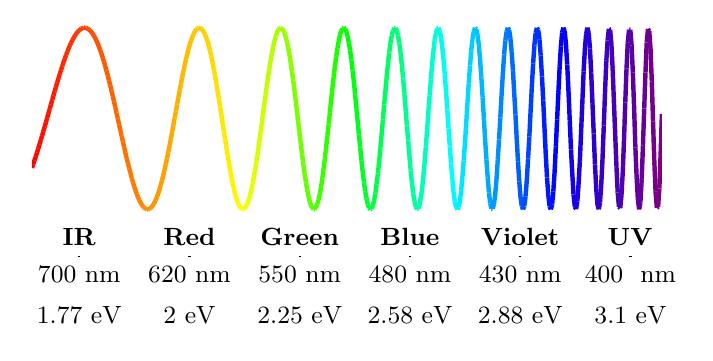
\begin{tikzpicture}
  % Rainbow plot using pgfplots with correct scale
  \begin{axis}[
    hide axis,
    scale=1,
    domain=2.6:3.6,
    samples=500,
    xmin=2.6, xmax=3.6,
    ymin=-0.26, ymax=0.26,
    scale only axis,
    width=8cm,
    height=3cm,
    every axis/.append style={scale=1}
  ]
    \addplot[
      mesh,
      ultra thick,
      point meta=x,
      colormap name=visiblespectrum
    ] {sin(deg(x^x))/5};
  \end{axis}
  
  % Horizontal bounds - adjusted with coordinates
  %\draw[dashed] (0.6,0.25) -- (8.6,0.25);
  %\draw[dashed] (0.6,-0.25) -- (8.6,-0.25);
  
  % Top labels: Color names
  \foreach \x/\pos/\label in {
    2.6/0.6/IR, 2.8/2.0/Red, 3.0/3.4/Green, 3.2/4.8/Blue, 3.4/6.2/Violet, 3.6/7.6/UV
  } {
    
    \node at (\pos,0) {\small \textbf{\label}};
    
  }
  
  % Bottom labels: nm values and calculated eV values
  \foreach \pos/\nm in {
    0.6/700, 2.0/620, 3.4/550, 4.8/480, 6.2/430, 7.6/400
  } {
    \draw[thick] (\pos,-0.26) -- (\pos,-0.25);
    \node[below] at (\pos,-0.26) {\small \nm~nm};
    
    % Calculate eV from nm: eV = 1240/nm
    \pgfmathparse{1240/\nm}
    \edef\ev{\pgfmathresult}
    \node[below=0.5cm] at (\pos,-0.26) {\small \pgfmathprintnumber[fixed, precision=2]{\ev}~eV};
    
  }
\end{tikzpicture}
\end{figure}

Platinum ($Z = 78$) also experiences strong relativistic shifts, but its partially filled 5d$^9$ configuration and broader interband spacing push absorption into the ultraviolet. Thus, platinum reflects visible light uniformly and appears silvery-white.

Copper ($Z = 29$), though far lighter, has a naturally narrow d–s gap of about 2.1 eV even without relativistic effects. This gap also falls within the visible range and leads to selective absorption of blue-green shades, producing its reddish hue.

Mercury ($Z = 80$) reveals a different consequence of relativistic orbital modifications. The 6s orbital contracts so strongly that its electrons become tightly bound and chemically inert. This reduces orbital overlap and weakens metallic bonding. The result is a low cohesive energy and a low melting point for a metal. Mercury remains liquid at room temperature — a phase behavior that non-relativistic models cannot reproduce.

\begin{commentary}[Commentary: Low-Limit Theories]
  Usually in physical sciences, there are simplifications to precise theories that are applicable when one "zooms out." For example, at low velocities, the Galilean formulation suffices without relativistic corrections. In low mass scenarios, Newtonian gravity replaces general relativity. These \textbf{"low-limit theories"} have well-defined domains of validity characterized by dimensionless parameters — velocity ratio ($v/c$), gravitational potential ($GM/rc^2$), or wavelength ratio ($\lambda/L$). When these parameters approach unity, the simplified theories break down.
  
  In mechanics one typically uses classical physics, and in chemistry, simplistic atomic models (electrons "orbiting" a nucleus) are adequate for most applications. \textbf{This is why it is remarkable that the color of gold requires relativistic corrections}. The relativistic effects on gold's electron orbitals cause it to absorb blue light and appear yellow, whereas non-relativistic predictions would yield a silvery appearance like its periodic table neighbors.
  
  It is rare to need special relativity for macroscopic phenomena we encounter daily. This makes gold particularly noteworthy — it represents one of the few cases where a common macroscopic property (color) can be correctly predicted only by including relativistic effects.
\end{commentary}